\chapter{PCP定理の証明} \label{chap:PCP-proof}

本チャプターはPCP定理の証明を与える.

\section{ギャップ増幅補題}
DinurによるPCP定理の証明は, 与えられた制約グラフの不満足値を段階的に増幅していくアプローチに基づく.
その中核を担うのがこのギャップ増幅補題であり, 制約グラフの不満足値を増幅できることを保証する補題である.
ギャップ増幅補題は以下のように述べられる.

\begin{lemma}{ギャップ増幅補題}{gap-amplification-lemma}
  二つの定数$c>0,\alpha\in (0,1)$, アルファベット$\Sigma$, および以下の性質を満たす決定的多項式時間アルゴリズム$A$が存在する: 
  アルゴリズム$A$は制約グラフ$G=\ip{(V,E),\Sigma,\calC}$を入力として受け取り, 次の性質を満たす別の制約グラフ$G'=\ip{(V',E'),\Sigma,\calC'}$を出力する:
  \begin{itemize}
    \item $\size(G')\le c\cdot \size(G)$.
    \item $\UNSAT(G)=0$ならば$\UNSAT(G')=0$.
    \item $\UNSAT(G)>0$ならば$\UNSAT(G')\ge \min\{\alpha, 2\cdot \UNSAT(G)\}$.
  \end{itemize}
\end{lemma}

PCP定理(\cref{thm:PCP-CSP-theorem})の証明は, この補題を繰り返し適用することによって得られる.

\begin{proof}[\cref{lem:gap-amplification-lemma}の下での\cref{thm:PCP-CSP-theorem}の証明.]
  3彩色問題のインスタンスを入力として受け取り, その制約グラフを$G_0$とし, 頂点数を$n$とする.
  この制約グラフは単純グラフであるため, $\UNSAT(G_0)=0$もしくは$\UNSAT(G_0)\ge \frac{1}{n^2}$である.
  \cref{lem:gap-amplification-lemma}のアルゴリズムを$A$とし, 各$i=1,\dots,\ceil{2\log_2 n}$について, 制約グラフ$G_i$を
  $G_i = A(G_{i-1})$として定義し, 最終的に得られる制約グラフを$G'=G_{\ceil{2\log_2 n}}$とする.
  各$G_i$のサイズは$\size(G_i) \le c\cdot \size(G_{i-1})$であるため, $\size(G')\le c^{\ceil{2\log_2 n}}\cdot \size(G_0)=\size(G_0)^{O(1)}$である.
  従って$G'$は多項式時間で構成できる.

  また, 不満足値については, 以下のようになる:
  \begin{itemize}
  \item もしも$G_0$がYesインスタンスであるならば, 全ての$i$に対して$G_i$もYesインスタンスであり, 特に$\UNSAT(G')=0$である.
  \item もしも$G_0$がNoインスタンスであるならば, $\UNSAT(G_0)\ge \frac{1}{n^2}$かつ$\UNSAT(G_i)\ge \min\{\alpha, 2\cdot \UNSAT(G_0)\}$であるため, $\UNSAT(G')\ge \min\qty{\alpha, 2^{2\log_2 n}\cdot \frac{1}{n^2}}=\alpha$である.
  \end{itemize}
\end{proof}


\section{制約グラフのべき乗}

\cref{lem:constant-degree-expanderization}により, 任意の制約グラフを定数次数エクスパンダーに変換することができる.
この節では, そのような制約グラフに対し, 以下で定義する\emph{べき乗}という操作を考えることで, その$\UNSAT$の値を増幅させることができることを示す.

\begin{definition}{制約グラフの冪乗}{power-of-constraint-graph}
  パラメータ$\ell\in\Nat$および全頂点が自己ループを持つ$d$-正則な制約グラフ$G=\ip{(V,E),\Sigma,\calC}$に対し, べき乗$G^\ell = \ip{(V,\boldE),\Sigma^{d^{\ell}},\calC^\ell}$を, 以下のようにして定義する:
  \begin{itemize}
    \item 頂点集合は同じ$V$とする. なお, $V$の元は$v_1<\dots < v_n$のように順序づけられているとする.
    \item グラフ$(V,\boldE)$をべき乗(\cref{def:power-of-graph})によって得られるグラフ$(V,E)^\ell$とする. すなわち, 各二頂点$u,v\in V$に対し, 長さ$\ell$の$uv$-路の個数と同じだけ$uv$間に多重辺を用意する ($uv$-路と$vu$路の個数は一致するため, 無向グラフとして定義できる). このようにして得られる辺の多重集合を$\boldE$とし, その元を$\bolde = \{u,v\} \in \boldE$とする.
    \item アルファベット集合は$\Sigma^{d^{\ell}}$とする. ここで, 頂点$u$に$\vec{\sigma}=(\sigma_1,\dots,\sigma_{d^{\ell}}) \in \Sigma^{d^{\ell}}$が割り当てられたとき, 次の意味を持つ: 元の$d$-正則グラフ$G$上で頂点$u$から距離$\ell$以内の頂点の集合を$\Gamma(u)$とし\footnote{頂点$v$が頂点$u$から距離$i$以内であるというのは, 頂点$u$から開始し頂点$v$に至る長さ$i$以下の路が存在することをいう.}, その元を頂点番号の大小順で並べて$\Gamma(u)=\qty{ v_1,\dots,v_\ell}$ とする (ここで$G$の$d$-正則性より$\ell \le d^{\ell}$である). このとき, $\vec{\sigma}$は各$v\in\Gamma(u)$に$\vec{\sigma}_u\in \Sigma$を割り当てる写像とみなし, $\vec{\sigma}_v$を\emph{$u$の$v$に対する意見}と呼ぶ.
    なお, $\ell < d^{\ell}$の場合は相異なる二つの$\vec{\sigma},\vec{\sigma}'\in\Sigma^{d^{\ell}}$が同一の写像としてみなされることもある (これらは制約を充足するか否かにおいては区別されない).
    \item 辺$\bolde = \{u,v\} \in \boldE$ に対応する制約$\boldc_{\bolde}\in \calC^\ell$は次の二つを満たす割り当て$(\vec{\sigma},\vec{\sigma}')\in \Sigma^{d^{\ell}} \times \Sigma^{d^{\ell}}$によって満たされる:
    元のグラフ$G$の全ての辺$e=\{s,t\}\in E$ (ただし$s<t$)に対し,
      \begin{itemize}
        \item $s\in \Gamma(u), t\in\Gamma(v)$ならば$(\vec{\sigma}(s), \vec{\sigma}'(t))\in c_e$が成り立つ.
        \item $s\in\Gamma(v), t\in\Gamma(u)$ならば$(\vec{\sigma}'(s), \vec{\sigma}(t))\in c_e$が成り立つ.
      \end{itemize}
  \end{itemize}
\end{definition}

\begin{figure}[ht]
  \centering
  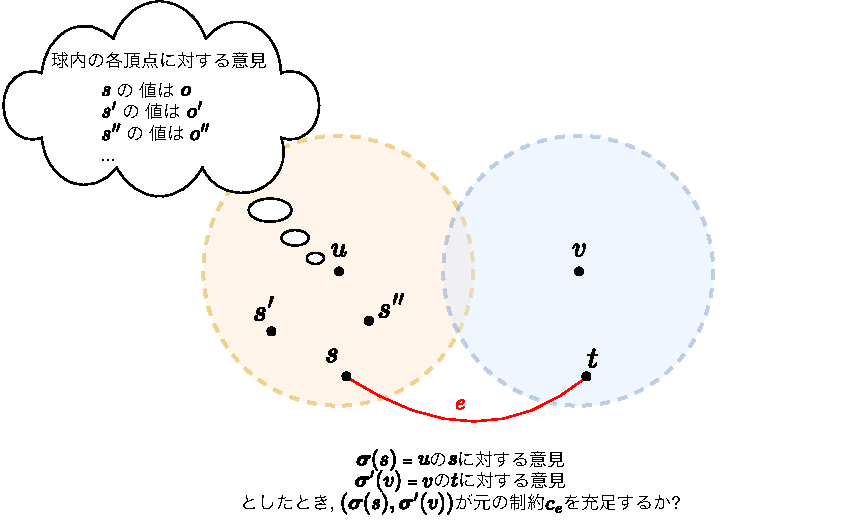
\includegraphics[width=\textwidth]{images/gap_amplification.pdf}
  \caption{制約グラフ$G$のべき乗$G^\ell$の図例. 頂点$u,v$にそれぞれ$\vec{\sigma},\vec{\sigma}'\in\Sigma^{d^{\ell}}$が割り当てられているとき, それぞれ関数$\vec{\sigma}\colon \Gamma(u)\to\Sigma$と$\vec{\sigma}'\colon \Gamma(v)\to\Sigma$とみなす. なお, 元のグラフ$G$が自己ループを持つことから, 距離$\ell$以内の全ての頂点に対して意見が定義される.\label{fig:gap-amplification}}
\end{figure}

パラメータ$\ell$は制約グラフのサイズ$\size(G)$には依存しない定数であることを常に想定する.
べき乗によって得られる制約グラフは元の制約グラフに対して$\UNSAT$の値が増幅する.

\begin{lemma}{べき乗の性質}{property-of-power}
  ある定数$\beta=\beta(\lambda,d,\abs{\Sigma})$が存在して以下が成り立つ:
  十分大きいパラメータ$\ell=\ell(d,\abs{\Sigma},\lambda) \le \abs{E}$および全頂点が自己ループを持つ$d$-正則な制約グラフ$G=\ip{(V,E),\Sigma,\calC}$に対し, べき乗$G^\ell = \ip{(V,\boldE),\Sigma^{\ell},\calC^\ell}$を, \cref{def:power-of-constraint-graph}で定義する.
  このとき
  \begin{itemize}
    \item $\size(G^\ell) \le \size(G)\cdot d^\ell$である.
    \item $\UNSAT(G)=0$ならば$\UNSAT(G^\ell)=0$である.
    \item $\UNSAT(G^\ell) \ge \beta\sqrt{\ell}\cdot \min\qty{ \UNSAT(G), \frac{1}{\ell} }$である.
  \end{itemize}
\end{lemma}

\begin{remark}{「定数」の意味}{mean-of-constants}
  主張や証明の中でしばし「定数」という言葉を多用するが, ここでは$d,\lambda,\abs{\Sigma}$をユニバーサルな定数で固定し, これらの値に応じて定まる値$\beta,\ell$なども定数と呼ぶ.
  ただし, 定数はグラフの頂点数や辺数には依存しない.
\end{remark}

\begin{proof}

定義より$\abs{\boldE} \le \abs{V}d^{\ell}$であるから, $\size(G^\ell) \le \size(G)\cdot d^\ell$である.

また, $\UNSAT(G)=0$ならば, 全制約を満たす割り当て$a\colon V \to \Sigma$に対し, $a'(u)$に
\begin{align*}
  \vec{\sigma}(u)\colon w \mapsto a(w)
\end{align*}
で定まる関数$\vec{\sigma}\colon \Gamma(w)\to\Sigma$とみなせる値$\vec{\sigma}\in\Sigma^{d^\ell}$を割り当てる (候補が複数存在する場合はどれでもよい).
このようにして定まる$a'\colon V\to\Sigma^{\ell}$を考えると, これは全ての制約を満たす割り当てであるため, $\UNSAT(G^\ell)=0$である.

最後に$\UNSAT(G^\ell)$の下界を証明する.
簡単のため$\ell$は偶数であるとする (奇数の場合は$\ell/2$を$\floor{\ell/2}$に置き換えれば同じ証明が成立する).
頂点$u\in V$に対し, $V$値をとる確率変数$\RW_j(u)$を, グラフ$G$上で頂点$u$から開始する長さ$j$のランダムウォークの最終到達頂点とする (長さとは辿った辺の本数のことである).
べき乗の制約グラフ$G^\ell$における割り当て$a'\colon V \to \Sigma^{\ell}$に対し, 元の制約グラフに対する任意の割り当て$a\colon V\to\Sigma$を
\begin{align}
  a(u) = \argmax_{\tau \in \Sigma} \qty{ \Pr\qty[ a'(\RW_{\ell/2}(u))_u = \tau ] }. \label{eq:argmax-of-RW}
\end{align}
によって定める.
常に$\RW_{\ell/2}(u)\in \Gamma(u)$であるから$a'(\RW(u))_u$は必ず存在する.
すなわち, $u$から開始したランダムウォークが最も「拾いやすい」意見を$a(u)$としている.
このようにして定めた割り当て$a\colon V \to \Sigma$は, 適当な定数$\beta=\beta(\lambda,d,\abs{\Sigma})>0$に対して
\begin{align}
  \UNSAT(a';G^\ell) \ge \beta\sqrt{\ell}\cdot \min\qty{ \UNSAT(a;G), \frac{1}{\ell} }. \label{eq:lower-bound-of-UNSAT}
\end{align}
を満たすことを後で示す. $\UNSAT(a';G^\ell)=\UNSAT(G^\ell)$を満たす$a'$に対して\cref{eq:lower-bound-of-UNSAT}を適用し, さらに$\UNSAT(a;G)\le \UNSAT(G)$を代入すると$\UNSAT(G^\ell)$の所望の下界が得られて証明は完了する.

\paragraph*{\cref{eq:lower-bound-of-UNSAT}の証明.}

割り当て$a'\colon V\to \Sigma^{d^{\ell}}$を固定し, $a$を\cref{eq:argmax-of-RW}によって定める.
辺部分集合$F_0\subseteq E$を, $a$によって充足されない辺の集合とし,
さらにその部分集合$F\subseteq F_0$を, 
\begin{itemize}
\item $\abs{F_0} \le \frac{\abs{E}}{\ell}$ならば$F_0=F$,
\item そうでない場合は$\abs{F} = \floor*{\frac{\abs{E}}{\ell}}$となるように$F$を任意に固定する.
\end{itemize}
このとき, 任意の$x\ge 1$に対し$\floor{x}\ge x/2$であることから, $\frac{\abs{E}}{\ell}\ge 1$の仮定を用いて
\begin{align}
  \abs{F} &\ge \min\qty{ \abs{F_0}, \floor*{\frac{\abs{E}}{\ell}} } \nonumber \\
  &\ge \frac{1}{2}\min\qty{ \abs{F_0}, \frac{\abs{E}}{\ell} } \nonumber \\
  &\ge \frac{\abs{E}}{2}\min\qty{ \UNSAT(a;G), \frac{1}{\ell} } \label{eq:abs-F}
\end{align}
を得る (なお, $\abs{E}\ge \ell$の仮定を用いるのはここのみである).

べき乗グラフの辺$\bolde \in \boldE$は$G$上の長さ$\ell$の路に対応する.
従って$\bolde = (u_0,\dots,u_\ell)$ (ただし全ての$i\in[\ell]$に対し$\qty{u_{i-1},u_{i}}\in E$)と表し, 元のグラフの辺と区別するため$e\in E$を$G$辺, $\bolde\in\boldE$を$G^\ell$辺と呼ぶことにする.

$G^\ell$辺$\bolde=(u_0,\dots,u_\ell)$の$i$番目の辺$e_i:=\qty{u_{i-1},u_i}$は
\begin{itemize}
  \item $e_i \in F$
  \item $a'(u_{0})_{u_{i-1}} = a(u_{i-1})$ かつ $a'(u_\ell)_{u_i} = a(u_i)$
\end{itemize}
をどちらも満たすとき, \emph{悪い}ということにする.
一様ランダムに$\bolde$を選んだとき, $B_i\in\binset$を辺$e_i$が悪いならば$B_i=1$, そうでないならば$B_i=0$とする (これらは確率変数である).
さらに
\begin{align*}
  I = \qty[\frac{\ell}{2} - \sqrt{\ell}, \frac{\ell}{2} + \sqrt{\ell}] \cap \mathbb{Z}
\end{align*}
に対し, $B=\sum_{i\in I}B_i$とする.
もしも$B>0$ならば, 辺$\bolde$の制約$c'_{\bolde}$は$a'$によって充足されない.
従って, $\UNSAT(a';G^\ell) \ge \Pr_{\bolde\sim \boldE}[B\ge 1]$である.

Paley-Zygmundの不等式(\cref{lem:paley-zigmund-inequality})より, $\E[B]$および$\E[B^2]$を評価することで$\Pr[B\ge 1]$の下界を得ることができる.
これらは以下のように評価できる. 

\begin{claim}{$B$の期待値}{expectation-of-B}
  ある十分小さな定数$C=C(d,\lambda,\abs{\Sigma})>0$が存在して, $B$の期待値は
  \begin{align*}
    \E[B] \ge C\sqrt{\ell} \cdot \frac{\abs{F}}{\abs{E}}.
  \end{align*}
\end{claim}

\begin{claim}{$B^2$の期待値}{expectation-of-B-squared}
  ある十分大きな定数$C'=C'(d,\lambda,\abs{\Sigma})>0$が存在して, $B^2$の期待値は
  \begin{align*}
    \E[B^2] \le C'\sqrt{\ell} \cdot \frac{\abs{F}}{\abs{E}}.
  \end{align*}
\end{claim}

これらの主張の証明は後で与える.
ここでは, これらを用いて\cref{eq:lower-bound-of-UNSAT}を示す.
実際, \cref{lem:paley-zigmund-inequality,claim:expectation-of-B,claim:expectation-of-B-squared}より, 定数$\beta=\frac{C^2}{2C'}>0$に対して
\begin{align*}
  \UNSAT(a';G^\ell) &\ge \Pr[B\ge 1] \\
  &\ge \frac{\E[B]^2}{\E[B^2]} \\
  &\ge \frac{C^2}{C'} \sqrt{\ell} \cdot \frac{\abs{F}}{\abs{E}} \\
  & \ge \beta \sqrt{\ell} \cdot \min\qty{ \UNSAT(a;G), \frac{1}{\ell} } & & \because \text{\cref{eq:abs-F}}
\end{align*}
となり主張を得る.

\end{proof}

最後に残された二つの主張の証明を与える. なお, 制約グラフのエクスパンダー性を用いるのは\cref{claim:expectation-of-B-squared}の証明のみである.
\begin{proof}[\cref{claim:expectation-of-B}の証明]
  各$i\in I$に対して$\E[B_i]=\Pr_{\bolde\sim \boldE}[e_i\text{ が悪い}]$を下から抑えればよい.
  一様ランダムな$\bolde=(u_0,\dots,u_\ell)\sim\boldE$は$G$上の長さ$\ell$のランダムウォークであるから, 各$i\in I$に対して$\bolde$は以下のプロセスによって生成される:
  \begin{enumerate}
    \item 辺$\{u_{i-1},u_i\}\sim E$を一様ランダムに選ぶ.
    \item 頂点$u_{i-1}$から開始して長さ$i-1$のランダムウォークを行い, 辿った頂点を順番に$u_{i-1},u_{i-2},\dots,u_0$とする.
    \item 同様に, 頂点$u_i$から開始して長さ$\ell-i$のランダムウォークを行い, 辿った頂点を順番に$u_i,u_{i+1},\dots,u_\ell$とする.
    \item 頂点列$(u_0,\dots,u_\ell)$に対応する$\bolde \in \boldE$を出力する.
  \end{enumerate}

  \begin{figure}[ht]
    \centering
    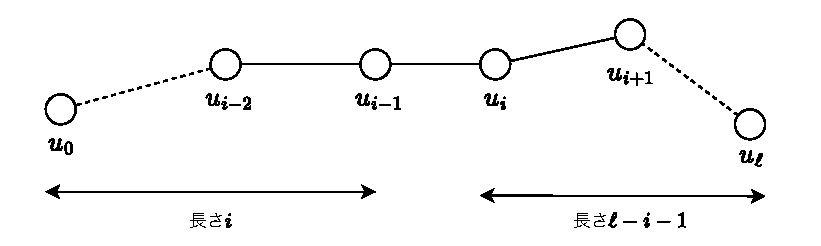
\includegraphics[width=0.9\textwidth]{images/randomwalk_process.pdf}
    \caption{ランダムウォークの図例. 頂点$u_0$から開始して長さ$i-1$のランダムウォークを行い, 辿った頂点を順番に$u_{i-1},u_{i-2},\dots,u_0$とする. 同様に, 頂点$u_i$から開始して長さ$\ell-i$のランダムウォークを行い, 辿った頂点を順番に$u_i,u_{i+1},\dots,u_\ell$とする. この二つのランダムウォークを組み合わせて, 長さ$\ell$のランダムウォークを生成する. \label{fig:random-walk}}
  \end{figure}

  このプロセスに基づいて, $\Pr[B_i=1]$を評価する.
  まず, ステップ1で選ばれた辺が$\qty{u_{i-1},u_i}\in F$である確率は$\frac{\abs{F}}{\abs{E}}$である.
  次にステップ1で選ばれた辺$\qty{u_{i-1},u_i}\in F$で条件つけたとき, ステップ2と3は独立なランダムネスに基づく試行であるため, それぞれの両端点$u_0,u_\ell$は独立な確率変数である.
  従って
  \begin{align}
    \Pr[B_i=1] &= \E_{\text{step 1-3}}\qty[\{u_{i-1},u_i\}\in F \text{ and }a'(u_0)_{u_{i-1}} = a(u_{i-1})\text{ and }a'(u_\ell)_{u_i} = a(u_i)] \nonumber \\
     &= \frac{\abs{F}}{\abs{E}} \cdot \E_{\{u_{i-1},u_i\}\sim F}\qty[ \underbrace{\Pr_{\text{step 2}}[a'(u_0)_{u_{i-1}} = a(u_{i-1})]}_{=:p_0} \cdot \underbrace{\Pr_{\text{step 3}}[a'(u_\ell)_{u_i} = a(u_i)]}_{=:p_\ell}] \label{eq:Pr-B_i}
  \end{align}
  を得る. 二つ目の等式では, $\{u_{i-1},u_i\}\in F$で条件つけて$\{u_{i-1},u_i\}\sim E$をランダムに選ぶというのは, $F$内の辺を一様ランダムに選ぶことに他ならないことに留意する.

  次に, $p_0$と$p_\ell$を評価する.
  頂点$u_{i-1}$を任意に固定して$p_0$を考える ($p_\ell$も同様に示せる).
  頂点$u\in V$および非負整数$m\ge 0$に対し, 確率変数$X_{u,m}\in\Sigma$を, ($a'$における)$\RW_m(u)$の$u$に対する意見, すなわち$X_{u,m} = a'(\RW_m(u))_u$とする.
  \cref{eq:argmax-of-RW}より, $m=\ell/2$のとき, 
  \begin{align}
  \Pr[X_{u_{i-1},\ell/2} = a(u_{i-1})] \ge \frac{1}{\abs{\Sigma}} \label{eq:center_opinion}
  \end{align}
  である.
  ステップ2で選ばれた端点$u_0$は$u_0=\RW_i(u_{i-1})$であるから, $X_{u_{i-1},i}=a'\qty( \RW_i(u_{i-1}) )_{u_{i-1}} = a'\qty(u_0)_{u_{i-1}}$である.
  従って, 
  \begin{align}
    p_0 = \Pr[X_{u_{i-1},i} = a(u_{i-1})] \label{eq:p_0}
  \end{align}
  である. 任意に頂点$u\in V$と$i\in I$を固定して$X_{u,\ell/2}$と$X_{u,i}$の分布を比較する.
  $i\in I$なので, $\abs{i-\ell/2} \le \sqrt{\ell}$である.

  元のグラフ$G$の各頂点に対し, その頂点が持つ自己ループの一つを赤く塗る
  (仮定より元のグラフ$(V,E)$は$d$-正則かつ各頂点が自己ループを少なくとも一つ持つ).
  頂点$u$から開始する長さ$\ell/2$のランダムウォークを考え,
  確率変数$Y_{\ell/2}$を, このランダムウォークが辿った赤\emph{以外}の辺の個数とする ($Y_i$も同様に定義する).
  各頂点がちょうど一つの赤い自己ループを持つため,
  確率変数$Y_{\ell/2}$の分布は始点$u$に依存せず二項分布$\Bin(\ell/2,1-1/d)$である (同様に$Y_i$の分布は$\Bin(i,1-1/d)$である).
  また, $\RW'_k(u)$を, 頂点$u$から開始する赤い辺を選ばない長さ$k$のランダムウォークの最終到達頂点とする (すなわち, $G$の各頂点から赤い辺を除いて得られるグラフ上の長さ$k$のランダムウォークである).
  従って, 任意の頂点部分集合$A\subseteq V$に対し
  \begin{align}
    \Pr\qty[\RW_{i}(u)\in A] &= \sum_{k=0}^{i} \Pr\qty[\RW_{i}(u) \in A \condition Y_{i}=k] \cdot \Pr\qty[Y_{i}=k] \nonumber \\
    &= \sum_{k=0}^{i} \Pr\qty[\RW'_k(u) \in A] \cdot \Pr\qty[Y_{i}=k] \label{eq:RW_i_distribution}
  \end{align}
  が成り立つ.
  ここで, 以下の主張を後で示す:
  \begin{claim}{}{two-constants}
  十分大きな定数$C_1=C_1(d,\abs{\Sigma})>0$と十分小さな定数$C_2=C_2(d,\abs{\Sigma})>0$が存在して以下が成り立つ:
  $K:= \qty{ k\in \mathbb{Z}_{\ge 0} \colon \abs{k - \qty(1-\frac{1}{d})\frac{\ell}{2}} \le C_1\sqrt{\ell} }$ としたとき,
  \begin{enumerate}
    \item $\Pr\qty[Y_{\ell/2} \not\in K] \le \frac{1}{2\abs{\Sigma}}$.
    \item 全ての$k\in K$と全ての$i\in I$に対し, $\Pr\qty[Y_i=k] \ge C_2\cdot \Pr\qty[Y_{\ell/2}=k]$.
  \end{enumerate}
  \end{claim}
  
  \cref{claim:two-constants}を仮定し, その定数$C_1,C_2$を用いて\cref{claim:expectation-of-B}を示す.
  パラメータ$\ell$は$d$に依存して十分大きくとる.
  このとき, 任意の$i\in I$に対して$K\subseteq [0,\ell/2-\sqrt{\ell}] \subseteq [0,i]$が成り立つから
  \begin{align}
    \Pr\qty[\RW_{i}(u)\in A] &= \sum_{k=0}^{i} \Pr\qty[\RW'_{k}(u) \in A] \cdot \Pr\qty[Y_{i}=k] \nonumber\\
    &\ge \sum_{k\in K} \Pr\qty[\RW'_{k}(u) \in A] \cdot \underbrace{\Pr\qty[Y_{i}=k]}_{\ge C_2\cdot \Pr\qty[Y_{\ell/2}=k]} \nonumber\\
    &\ge C_2 \sum_{k \in K} \Pr\qty[\RW'_{k}(u) \in A] \cdot \Pr\qty[Y_{\ell/2}=k] \nonumber\\
    &\ge C_2 \qty(\sum_{0\le k \le \ell/2} \Pr\qty[\RW'_{k}(u) \in A] \cdot \Pr\qty[Y_{\ell/2}=k] - \Pr[Y_{\ell/2}\not\in K]) \nonumber\\
    &\ge C_2 \qty( \Pr\qty[ \RW_{\ell/2}(u)\in A ] - \frac{1}{2\abs{\Sigma}} ) \label{eq:RW_i_distribution_2}
  \end{align}
  を得る. ここで頂点部分集合$A\subseteq V$を
  $A = \qty{ v \in V \colon a'(v)_u = a(u) }$
  として\cref{eq:RW_i_distribution_2}を適用すると
  \begin{align*}
    \Pr\qty[X_{u,i}=a(u)] = \Pr\qty[ a'\qty(\RW_{i}(u))_u = a(u) ] = \Pr\qty[\RW_{i}(u)\in A] \ge \frac{C_2}{2\abs{\Sigma}}
  \end{align*}
  となるため, $u=u_{i-1}$とすると, \cref{eq:p_0}より
  \begin{align*}
    p_0 = \Pr\qty[X_{u_{i-1},i} = a(u_{i-1})]\ge \frac{C_2}{2\abs{\Sigma}}
  \end{align*}
  を得る.
  同様に, $p_\ell$についても, 適当な定数$C'_2>0$に対して$p_{\ell}\ge \frac{C'_2}{2\abs{\Sigma}}$が成り立つため, \cref{eq:Pr-B_i}より, 適当な定数$C_3=C_3(d,\abs{\Sigma})>0$に対して
  \begin{align*}
    \Pr[B_i=1] &\ge \frac{\abs{F}}{\abs{E}} \cdot \E_{\{u_{i-1},u_i\}\sim F}\qty[ p_0 \cdot p_\ell ] \ge C_3\cdot \frac{\abs{F}}{\abs{E}}
  \end{align*}
  を得る. 最後に$B=\sum_{i\in I}B_i$より, $\E[B]\ge C_3\sqrt{\ell}\cdot \frac{\abs{F}}{\abs{E}}$を得る.
\end{proof}

\begin{proof}[\cref{claim:two-constants}の証明]
  一つ目の主張は, $Y_{\ell/2}$の分布が二項分布$\Bin(\ell/2,1-1/d)$であることとChebyshevの不等式(\cref{lem:chebyshev-inequality})を用いれば示せる (\cref{exer:two-constants}).

  二つ目の主張を示す. すなわち, 二つの二項分布$\Bin(i,1-1/d)$と$\Bin(\ell/2,1-1/d)$を比較する.
  一つ目の主張を満たすように任意に定数$C_1>0$を固定する.
  このとき, 二つ目の主張が成り立つようにうまく$C_2>0$を選べることを示せばよい.

  一般に, 任意の$m\in\Nat$, 定数$p\in(0,1)$, $C>0$および$k\in\Nat$ (ただし$\abs{k-mp}\le C\sqrt{m}$を満たす)に対し, 
  \begin{align}
    \Pr\qty[\Bin(m,p) = k] = \frac{1}{\sqrt{2\pi m p(1-p)}} \exp\qty( - \frac{(k-mp)^2}{2m p(1-p)} ) \cdot \qty(1\pm O_{C,p}\qty(\frac{1}{m})) \label{eq:de-moivre-laplace}
  \end{align}
  が成り立つ (De Moivre-Laplaceの定理).
  特に, $\abs{k-mp}\le C\sqrt{m}$を満たすため, 右辺は$\Theta(1/\sqrt{m})$で評価できる.
  
  従って, 適当な定数$D_1,D_2>0$が存在して, $\ell$が十分大きいとき,
  \begin{align*}
    &\Pr[Y_i=k]=\Pr[\Bin(i,1-1/d)=k] \ge \frac{D_1}{\sqrt{i}}, \\
    &\Pr[Y_{\ell/2}=k]=\Pr[\Bin(\ell/2,1-1/d)=k] \le \frac{D_2}{\sqrt{\ell/2}}
  \end{align*}
  を満たす. $i\in I$より, 主張を得る.    
\end{proof}

\begin{exercise}{主張の証明}{two-constants}
  \cref{claim:two-constants}の一つ目の主張, すなわちある十分大きな定数$C_1=C_1(d,\abs{\Sigma})>0$が存在して
  \begin{align*}
    \Pr\qty[Y_{\ell/2} \not\in K] \le \frac{1}{2\abs{\Sigma}}
  \end{align*}
  が成り立つことを示せ.
\end{exercise}

\begin{proof}[\cref{claim:expectation-of-B-squared}の証明]
  ランダムウォーク$\bolde=(u_0,\dots,u_\ell)\sim\boldE$に対し, 確率変数$Z_i$を, $\qty{u_{i-1},u_i}\in F$ならば$Z_i=1$, そうでなければ$Z_i=0$とする.
  このとき, $B_i\le Z_i$であるから, $Z:=\sum_{i\in I} Z_i$に対し$B\le Z$であり, 特に$\E[B^2]\le \E[Z^2]$である.
  以下, $\E[Z^2]$を評価する. まず, $\E[Z_i]=\Pr[\qty{u_{i-1},u_i}\in F]=\frac{\abs{F}}{\abs{E}}$である (ランダムウォークの$i$番目の辺の周辺分布は$E$上の一様分布だから).
  定義より
  \begin{align}
    \E[Z^2] &= \sum_{i,j\in I} \E[Z_i Z_j] = \E[Z] + 2 \sum_{i,j\in I,i<j} \E[Z_i Z_j] \nonumber \\
    &= \frac{\abs{F}}{\abs{E}} \abs{I} + 2 \sum_{i,j\in I,i<j} \E[Z_iZ_j]. \label{eq:E-Z^2}
  \end{align}
  ここで, 固定した$i<j$に対して$\E[Z_iZ_j]$を上から評価する.
  すなわち, $\lambda$-エクスパンダーグラフ上の長さ$\ell$のランダムウォーク$(u_0,\dots,u_\ell)$を考えたとき, $i$番目の辺$\qty{u_{i-1},u_i}$と$j$番目の辺$\qty{u_{j-1},u_j}$が同時に$F$に含まれる確率を評価する.
  辺部分集合$F\subseteq E$の辺に接続している頂点部分集合を$V_F:=\bigcup_{e\in F} e$とすると
  \begin{align}
    \Pr_{(u_{i-1},\dots,u_j)}\qty[\qty{u_{i-1},u_i}\in F \text{ and } \qty{u_{j-1},u_j}\in F] \le \Pr_{(u_{i-1},\dots,u_j)}\qty[u_{i-1}\in V_F\text{ and }u_j\in V_F] \label{eq:V_F-bound}
  \end{align}
  となる. ここでは, 頂点$u_{i-1}$を一様ランダムに選び, そこから開始する長さ$j-i+1$のランダムウォーク$(u_{i-1},u_i,\dots,u_{j-1},u_j)$に関する確率を考えている.
  このランダムウォークは, べき乗グラフ$G^{j-i+1}$上の長さ$1$のランダムウォークと一致する.
  \cref{lem:power-of-regular-expander}より, $G^{j-i+1}$は$d^{j-i+1}$-正則かつ$\lambda^{j-i+1}$-エクスパンダーである.
  従って, \cref{lem:expander-mixing-lemma}より, \cref{eq:V_F-bound}の右辺は
  \begin{align*}
    \Pr\qty[u_{i-1}\in V_F\text{ and }u_j\in V_F] &= \frac{W(V_F,V_F)}{nd^{j-i+1}} \\
    &\le \qty(\frac{\abs{V_F}}{n})^2 + \lambda^{j-i+1} \cdot \frac{\abs{V_F}}{n} \\
    &\le \qty(\frac{2\abs{F}}{n})^2 + \lambda^{j-i+1} \cdot \frac{2\abs{F}}{n} \\
    &= \frac{d\abs{F}^2}{\abs{E}^2} + \frac{\lambda^{j-i+1}d\abs{F}}{\abs{E}}
  \end{align*}
  を得る. ここで,
  $\abs{F}/\abs{E} \le 1/\ell$および$\abs{I} \le 2\sqrt{\ell}$を用いると,
  ある定数$C=C(d,\lambda)>0$が存在して
  \begin{align*}
    \sum_{i,j\in I,i<j} \E[Z_iZ_j] &\le d\underbrace{\abs{I}^2 \qty(\frac{\abs{F}}{\abs{E}})^2}_{\le 4\abs{F}/\abs{E}} + \frac{d\abs{F}}{\abs{E}} \sum_{i,j\in I,i<j} \lambda^{j-i+1} \\
    &\le 4d \frac{\abs{F}}{\abs{E}} + d\abs{I}\cdot \frac{\abs{F}}{\abs{E}} \cdot \sum_{i\ge 0} \lambda^i \\
    &\le C\abs{I}\frac{\abs{F}}{\abs{E}}.
  \end{align*}
  これと\cref{eq:E-Z^2}を組み合わせると, 主張を得る.
\end{proof}

\section{アルファベット削減}
ギャップ増幅補題(\cref{lem:gap-amplification-lemma})では変換前後で制約グラフのアルファベットは同一であることを主張しているが,
べき乗をとることによって, $\UNSAT$の値は$\sqrt{\ell}$倍に増幅する一方でアルファベットは$\Sigma^\ell$になってしまう.
そこで, アルファベット$\Sigma^\ell$上の制約グラフ$G$を, $\UNSAT$や$\size$をそれほど損なわずアルファベット$\Sigma$上の制約グラフ$G'$に変換する必要がある.
\begin{theorem}{アルファベット削減}{alphabet-reduction}
  ある定数$\gamma>0$, アルファベット$\Sigma_0$, および多項式時間アルゴリズム$A$が存在して以下が成り立つ:
  アルゴリズム$A$は制約グラフ$G=\ip{(V,E),\Sigma,C}$を入力として受け取り,
  別の制約グラフ$G'=\ip{(V',E'),\Sigma_0,C'}$を出力する.
  ただし$G'$は, ある定数$c=c(\abs{\Sigma})>0$に対して
  \begin{itemize}
    \item $\size(G') \le c\cdot \size(G)$
    \item $\UNSAT(G)=0$ならば$\UNSAT(G')=0$
    \item $\UNSAT(G)>0$ならば$\UNSAT(G') \ge \gamma\UNSAT(G)$
  \end{itemize}
\end{theorem}
\cref{thm:alphabet-reduction}の証明では,
  まず, あるアルファベット$\Sigma_1$と定数$k\in\Nat$が存在して,
  与えられた制約グラフ$G=\ip{(V,E),\Sigma,\calC}$を, アルファベット$\Sigma_1$上の$k$-CSP $\varphi=\ip{(X,\Sigma_1,\calI,\calC')}$に変換する多項式時間アルゴリズム$A'$が存在することを示す.
  次にこの$k$-CSPを\cref{lem:k-CSP-constraint-graph-representation}を用いて$\Sigma_0:=\Sigma_1^k$上の制約グラフ$G'=\ip{(V',E'),\Sigma_0,\calC'}$に変換することによって証明は完了する.

\begin{lemma}{}{alphabet-reduction-kCSP}
  ある定数$q_0\in\Nat$と多項式時間アルゴリズム$A'$が存在して以下が成り立つ:
  任意のアルファベット$\Sigma$に対し, ある定数$c=c(\abs{\Sigma})>0$が存在し,
  アルゴリズム$A'$は制約グラフ$G=\ip{(V,E),\Sigma,C}$を入力として受け取り,
  $q_0$-CSP $\varphi=(X,\binset,\calI,\calC')$を出力する.
  ただし, $\varphi$は
  \begin{itemize}
    \item $\abs{X} \le c\cdot\size(G)$, $\abs{\calI} \le c\cdot\size(G)$.
    \item $\UNSAT(G)=0$ならば$\UNSAT(\varphi)=0$.
    \item $\UNSAT(G)>0$ならば$\UNSAT(\varphi) \ge 0.99\cdot\UNSAT(G)$.
  \end{itemize}
\end{lemma}
\begin{proof}
  $b = \ceil{\log_2\abs{\Sigma}}$とし, アルファベット$\Sigma$を$\binset^b$と同一視する
  ($\abs{\Sigma}$が2ベキでない場合はダミーの値を追加して$\abs{\Sigma}=\binset^b$とし, 各制約はダミーの値を読み込んだ場合は常に拒否するようにすればよい).
  制約グラフ$G$の各辺$e\in E$に対応する制約$c_e\subseteq \Sigma^2$を指示関数$c_e\colon\Sigma^2\to\binset$と同一視し, これを二入力の論理回路として表現したものを$C_e\colon \binset^b\times \binset^b\to \binset$とする.

  \begin{figure}[ht]
    \centering
    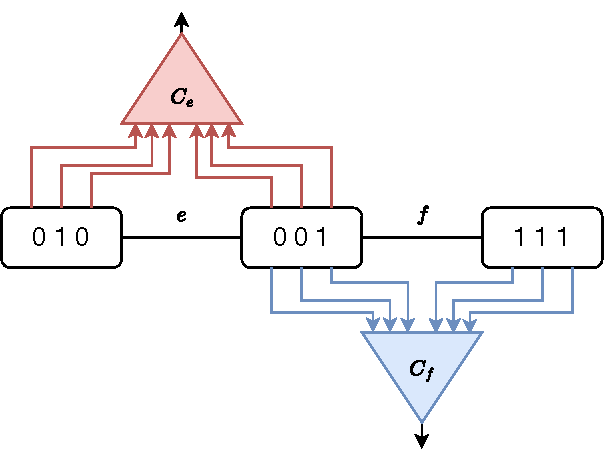
\includegraphics[width=0.8\textwidth]{images/newCSP.pdf}
    \caption{$2$-CSPの各辺の制約を論理回路として表現したもの. \label{fig:newCSP}}
  \end{figure}

  各辺$e=\qty{u,v}\in E$に対し, このようにして得られた各$C_e$に対して\cref{thm:two-input-circuit-PCP}を適用する.
  この定理から得られる検証者$V^{\pi_u,\pi_v,\pi_e}(C_e)$に対し,
  ランダムシード$r\in\binset^{\poly(b)}$を固定したときの決定的な検証者を$V^{\pi_u,\pi_v,\pi_e}(C_e;r)$とする. なお, $V$の時間計算量は高々$\poly(b)\le T$であるとする.
  これは以下の性質を持つ:
  \begin{itemize}
    \item $C_e(\sigma_u,\sigma_v)=1$を満たす$\sigma_u,\sigma_v\in\binset^b$に対して $\pi_u=\Had_b(\sigma_u)$および$\pi_v=\Had_b(\sigma_v)$であるならば, ある$\pi_e\in \F_2^{2^{2b} + 2^{4b^2}}$が存在して, 全ての$r\in\binset^T$に対して$V^{\pi_u,\pi_v,\pi_e}(C_e;r)$は受理する.
    \item $C_e(\sigma_u,\sigma_v)=1$を満たす任意の$\sigma_u,\sigma_v\in\binset^b$に対して$\dist(\pi_u,\Had_b(\sigma_u))\ge0.01$または$\dist(\pi_v,\Had_b(\sigma_v))\ge0.01$を満たす任意の$\pi_u,\pi_v$および任意の$\pi_e \in \F_2^{2^{2b} + 2^{4b^2}}$に対して, $\Pr_r\qty[V^{\pi_u,\pi_v,\pi_e}(C_e;r)\text{ rejects}]\ge 0.99$である.
    \item ある定数$q=O(1)$が存在して検証者$V^{\pi_u,\pi_v,\pi_e}(C_e)$は高々$q$回のオラクルアクセスを行う. なお, 最終的に構成するCSPは$q$-CSPとなる.
  \end{itemize}
  
  \begin{figure}[ht]
    \centering
    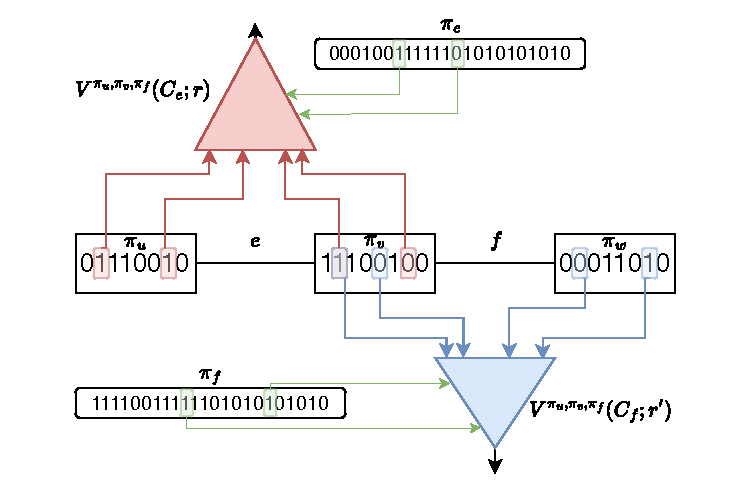
\includegraphics[width=\textwidth]{images/newCSP2.pdf}
    \caption{構成する$q_0$-CSPの図. PCPP検証者がアクセスするオラクルを文字列とみなした時の各成分が変数に対応する. 実際には, 各$r\in\binset^T$に対して$V^{\pi_u,\pi_v,\pi_e}(C_e;r)$を列挙してそれらを全て制約に追加する. \label{fig:newCSP2}}
  \end{figure}
  
  最終的に出力する新しい$q_0$-CSP $\varphi$を以下のように構成する.
  \begin{itemize}
    \item 各$u\in V$と各$i\in \qty[2^b]$に対し, $\pi_{u,i}\in\F_2$を変数とする. また, $\pi_u=\qty(\pi_{u,i})_{i\in[2^b]}\in \F_2^{2^b}$とする. 同様に, 各$e\in E$と各$j\in \qty[ 2^{2b} + 2^{4b^2} ]$に対し, $\pi_{e,j}\in\F_2$を変数とする. また, $\pi_e=\qty(\pi_{e,j})_{j\in\qty[2^{2b} + 2^{4b^2}]}\in \F_2^{2^{2b} + 2^{4b^2}}$とする. 全体の変数集合は$X=\qty{\pi_{u,i}\colon u\in V,i\in[2^b]} \cup \qty{\pi_{e,j}\colon e\in E,j\in[2^{2b} + 2^{4b^2}]}$となる.
    \item 各$e=\qty{u,v}\in E$と各$r\in\binset^{T}$に対し, 「$V^{\pi_u,\pi_v,\pi_e}(C_e;r)=1$」という制約を$c'_{e,r}$とし, $e\in E,r\in\binset^T$全てに対して$c'_{e,r}$を集めたものを$\calC'$とする. この検証者$V^{\pi_u,\pi_v,\pi_e}(C_e;r)$は, 変数$\pi_u,\pi_v,\pi_e$をオラクルとして実行する.
  \end{itemize}
  各制約「$V^{\pi_u,\pi_v,\pi_e}(C_e;r)=1$」は, 検証者が高々$q_0$回のオラクルアクセスを行うことから, 高々$q_0$個の変数の値に依存する. すなわち$\varphi$は$q_0$-CSPである.

  この$q_0$-CSP $\varphi$が所望の性質を満たすことを以下で確認する.
  \paragraph*{$\varphi$のサイズ.}
  頂点(変数)の個数は$2^b\cdot\abs{V} + \abs{E}\cdot\qty(2^{2b} + 2^{4b^2}) \le c\cdot\size(G)$であり,
  制約の個数は$2^T\cdot\abs{E} \le 2^{\poly(b)}\cdot\abs{E}$である (検証者の時間計算量が$b$に関して多項式で抑えられることから$T\le\poly(b)$である).
  
  \paragraph*{充足割り当ての存在性.}
  $G$の制約全てを満たす制約$a\colon V\to\Sigma$が存在すると仮定する.
  このとき, 各$u\in V$に対して
  \begin{align*}
    \pi_u = \Had_b(a(u))
  \end{align*}
  とする. このとき, 各辺$e=\qty{u,v}\in E$に対して$(a(u),a(v))$は辺$e$における制約を充足する.
  従って, \cref{thm:two-input-circuit-PCP}より, ある$\pi_e\in \F_2^{2^{2b} + 2^{4b^2}}$が存在して, 全ての$r\in\binset^T$に対して$V^{\pi_u,\pi_v,\pi_e}(C_e;r)$は受理する.
  このように構成された$(\pi_u)_{u\in V}$と$(\pi_e)_{e\in E}$から定まる$\varphi$の割り当て$a'\colon X\to \binset$は$\varphi$の制約全てを充足する.

  \paragraph*{不満足値の性質.}
 $\UNSAT(\varphi)\ge 0.99\cdot\UNSAT(G)$を示す.
  $\varphi$の任意の割り当て$a'\colon X\to\binset$を固定する.
  各頂点$u\in V$に対し, $a'$が定める
  変数$\pi_u$に対する部分割り当ての値を$\pi'_u\in\binset^b$とする.
  元の制約グラフ$G$の各頂点$u\in V$に対し, $a(u)\in\Sigma$を「$\pi'_u$の復号化」, すなわち
  \begin{itemize}
    \item ある$\sigma\in\Sigma$が存在して$\dist(\pi'_u,\Had_b(\sigma)) \le 0.01$ならば, $a(u)=\sigma$ (このような$\sigma$は存在するならば一意であることが\cref{exer:uniqueness-of-nearest-linear-function}から保証されている)
    \item そうでないならば, $a(u)\in\Sigma$は任意に選ぶ
  \end{itemize}
  で定める.
  辺部分集合$F\subseteq E$を$\UNSAT(a;G)$に寄与する辺の集合とする. すなわち, 辺$e=\qty{u,v}\in E$であって, $(a(u),a(v))$が辺$e$における制約を充足しないようなものの集合とする.

  任意の$e=\qty{u,v}\in E$に対して, $\dist(\pi'_u,\Had_b(\sigma_u))\le0.01$かつ$\dist(\pi'_v,\Had_b(\sigma_v))\le0.01$を満たす$(\sigma_u,\sigma_v)\in c_e$が存在するならば, 
  $a(u)=\sigma_u$かつ$a(v)=\sigma_v$であるため, $e\not\in F$となる.
  対偶をとると, 任意の$e=\qty{u,v}\in F$と
    任意の$(\sigma_u,\sigma_v)\in c_e$に対して, $\dist(\pi'_u,\Had_b(\sigma_u))>0.01$または$\dist(\pi'_v,\Had_b(\sigma_v))>0.01$が成り立つことがわかる.
  
  従って, 検証者$V(C_e)$の性質(\cref{thm:two-input-circuit-PCP})より, 任意の$e\in F$に対して
  \begin{align*}
    \forall \pi'_e \in \binset^{2^{2b} + 2^{4b^2}},\quad \Pr_{r\sim\binset^T}\qty[ V^{\pi'_u,\pi'_v,\pi'_e}(C_e;r)\text{が拒否する} ] \ge 0.99
  \end{align*}
  が成り立つ.
  すなわち, $e\in F$に関する$2^T$個の制約のうち, $0.99\cdot 2^T$個の制約は割り当て$\pi_u\leftarrow \pi'_u,\,\pi_v\leftarrow \pi'_v,\,\pi_e\leftarrow \pi'_e$に対して充足されない.
  従って,
  \begin{align*}
    \UNSAT(a';\varphi) &= \Pr_{e\sim E,r\sim\binset^T}\qty[ V^{\pi_u,\pi_v,\pi_e}(C_e;r)\text{が拒否する} ] \\
    &= \Pr_{e\sim E,r\sim\binset^T}\qty[ V^{\pi_u,\pi_v,\pi_e}(C_e;r)\text{が拒否する} \condition e\in F ]\cdot\Pr\qty[e\in F] \\
    &\ge 0.99\cdot \frac{\abs{F}}{\abs{E}} \\
    &= 0.99\cdot \UNSAT(a;G)
  \end{align*}
  が成り立つ.
\end{proof}

最後に\cref{lem:k-CSP-constraint-graph-representation}を用いて, $q_0$-CSPを制約グラフ$G'=\ip{(V',E'),\Sigma_0,\calC'}$に変換して証明が完了する:
\begin{proof}[\cref{thm:alphabet-reduction}の証明.]
  入力として受け取った制約グラフ$G=\ip{(V,E),\Sigma,\calC}$に対し, \cref{lem:alphabet-reduction-kCSP}を用いて, アルファベット$\binset$上の$q_0$-CSPのインスタンス $\varphi=\ip{(X,\binset,\calI,\calC')}$を構成する (これは多項式時間で行える).
  さらにこの$q_0$-CSPインスタンス$\varphi$を, \cref{lem:k-CSP-constraint-graph-representation}を用いて制約グラフ$G'=\ip{(V',E'),\binset^{q_0},\calC''}$に変換する.
  アルゴリズム$A$はこのようにして得られる制約グラフ$G'$を出力する.

  以下に$G'$が所望の性質を持つことを確認する:
  まず, \cref{lem:alphabet-reduction-kCSP}より, ある定数$c=c(\abs{\Sigma})>0$が存在して, $\varphi$は
  \begin{itemize}
    \item $\abs{X} \le c\cdot\size(G)$, $\abs{\calI} \le c\cdot\size(G)$.
    \item $\UNSAT(G)=0$ならば$\UNSAT(\varphi)=0$.
    \item $\UNSAT(G)>0$ならば$\UNSAT(\varphi) \ge 0.99\cdot\UNSAT(G)$.
  \end{itemize}
  が成り立つ.
  このとき, \cref{lem:k-CSP-constraint-graph-representation}より, $G'$はアルファベット$\binset^{q_0}$上の制約グラフであって, $q_0$のみに依存するある定数$c'$に対して
  \begin{itemize}
    \item $\size(G') \le c'q_0\cdot (\abs{X} + \abs{\calI})$.
    \item $\UNSAT(\varphi)=0$ならば$\UNSAT(G')=0$.
    \item $\UNSAT(\varphi)>0$ならば$\UNSAT(G') \ge \frac{1}{q_0}\cdot\UNSAT(\varphi)$.
  \end{itemize}
  が成り立つ.
  これらを組み合わせると
  \begin{itemize}
    \item $\size(G') \le c\cdot c'q_0\cdot\size(G)$
    \item $\UNSAT(G)=0 \Rightarrow \UNSAT(\varphi)=0\Rightarrow \UNSAT(G')=0$.
    \item $\UNSAT(G') \ge \frac{1}{q_0}\cdot \UNSAT(\varphi) \ge \frac{0.99}{q_0}\cdot \UNSAT(G)$
  \end{itemize}
  が成り立つ.
\end{proof}

\section{PCP定理の証明}
PCP定理を証明する全ての準備が整った.
\begin{proof}[\cref{thm:PCPtheorem}の証明.]
  ...
\end{proof}